\documentclass[smaller,aspectratio=169,ignorenonframetext,compress,sans,fleqn,xcolor=dvipsnames,fleqn,table,stillsansserifmath,stillsansseriftext,stillsansserifsmall,stillsansseriflarge]{beamer} 

\usepackage[utf8]{inputenc} 
\usepackage[T1]{fontenc}
\usepackage{xcolor}
\usepackage{framed}
\useoutertheme[height=0pt,width=35pt,hideallsubsections]{sidebar}
\definecolor{myblue}{HTML}{3b5998}
\definecolor{lightblue}{HTML}{8b9dc3}

\beamertemplateboldtitlepage
\beamertemplateboldframetitle

\beamertemplatenumberedsectiontoc

\beamertemplatenavigationsymbolsempty
\beamertemplatetransparentcovered

\setbeamercovered{invisible}
\setbeamercolor{alerted text}{fg=blue}

\usesectionheadtemplate
  {\insertsectionhead\hfill}
  {\color{fg!50!bg}\insertsectionhead\hfill}


\mode<article>{\usepackage{fullpage}}
\mode<article>{\renewcommand{\note}[1]{#1}}

\usepackage{intro}
\usepackage{definitions}

\setbeamercolor{sidebar}{bg=myblue}
\setbeamercolor{structure}{fg=myblue}

\usepackage{animate}

\usepackage{bbding}


\tikzstyle{point}=[circle, draw, fill=black!50,
                        inner sep=0pt, minimum width=4pt]
\newcommand{\plotpoints}{
  \draw node[point] (a) at (1,2) {};% \node[above=2pt of a] {$a$};
  \draw node[point] (b) at (3,0) {};% \node[above=2pt of b] {$b$};
  \draw node[point] (c) at (4,1) {};% \node[above=2pt of c] {$c$};
  \draw node[point] (d) at (7,0) {};% \node[above=2pt of d] {$d$};
  \draw node[point] (e) at (6,2) {};% \node[above=2pt of e] {$e$};
  \draw node[point] (f) at (7,4) {};% \node[above=2pt of f] {$f$};
  \draw node[point] (g) at (3,4) {};% \node[above=2pt of g] {$g$};
}

\graphicspath{{Figures/}}


\title{}



\begin{document}

%%%%% Formalities %%%%%

\begin{frame}[label=firstpage]
\frametitle{DM865 --- Heuristics and Approximation Algorithms}

\begin{tabular}{ll}
  {\alert{Teachers:}}
  & Marco Chiarandini \& Lene Favrholdt \\[2mm]

{\alert{Credits:}}
& 10 ECTS\\[-1mm]

\parbox[t]{0pt}{\alert{Prerequisites:}}
& \begin{minipage}[t]{0.72\textwidth}
    \begin{itemize}
    \item[\CheckmarkBold] Programming (DM502, DM503, DM550)
    \item[\CheckmarkBold] Algorithms and Datastructures (DM507)
    \item[\color{gray}\Checkmark] Complexity and Computability (DM508, DM553)
    \item[\color{gray}\Checkmark] Linear and Integer Programming (DM559, DM545, DM554, DM871)
    \end{itemize}
  \end{minipage}\\

&\\[-1mm]

{\alert{Language:}}
& English and/or Danish\\[2mm]

{\alert{Classes:}}
& Intro: $2h\times 20$; training: $2h\times 15$ \\[2mm]

{\alert{Material:}}
& Slides + textbook + articles + starting code\\[2mm]

{\alert{Assessment:}}
& Practical projects + oral exam
\end{tabular}
\end{frame}



%%%%% Contents%%%%%
\begin{frame}
\frametitle{Approximation Algorithms}
\framesubtitle{A $2$-approximation algorithm for Metric TSP: Double-Tree}

\begin{framed}
Double tree algorithm:
\medskip
\begin{enumerate}
\item $T\leftarrow \text{MST}$
\item Double all edges in $T$
\item  $E_{tour} \leftarrow$ Euler tour
\item $\text{Tour}\leftarrow$ vertices in order of appearance in $E_{tour}$
\end{enumerate}
\end{framed}


\bigskip


\begin{columns}[T,onlytextwidth]

  \column{0.3\textwidth}
  \centering
  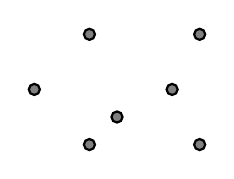
\begin{tikzpicture}[thick,scale=0.35]
    \plotpoints
  \end{tikzpicture}
  
  \column{0.3\textwidth}
  \centering
  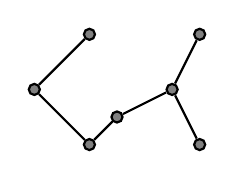
\begin{tikzpicture}[thick,scale=0.35]
    \plotpoints
    \draw (a) -- (b) -- (c) -- (e) -- (d);
    \draw (e) -- (f);
    \draw (a) -- (g);
  \end{tikzpicture}
  \column{0.3\textwidth}
  \centering
  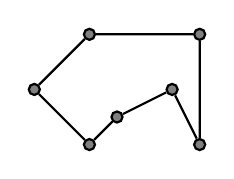
\begin{tikzpicture}[thick,scale=0.35]
    \plotpoints
    \draw (a) -- (b) -- (c) -- (e) -- (d)  -- (f) -- (g) -- (a);
  \end{tikzpicture}

\end{columns}

\end{frame}



\begin{frame}
\frametitle{Approximation Algorithms}
\framesubtitle{A $2$-approximation algorithm for Metric TSP: Double-Tree}

\bigskip

\begin{columns}[T,onlytextwidth]

  \column{0.3\textwidth}
  \centering
  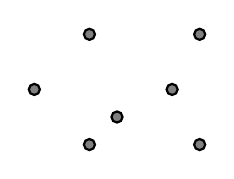
\begin{tikzpicture}[thick,scale=0.35]
    \plotpoints
  \end{tikzpicture}
  
  \column{0.3\textwidth}
  \centering
  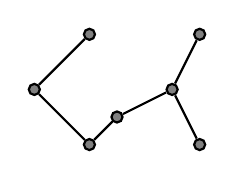
\begin{tikzpicture}[thick,scale=0.35]
    \plotpoints
    \draw (a) -- (b) -- (c) -- (e) -- (d);
    \draw (e) -- (f);
    \draw (a) -- (g);
  \end{tikzpicture}

  \bigskip

  MST
  \[
    c(\text{MST})\leq c(\text{OPT}):
  \]

  \column{0.3\textwidth}
  \centering
  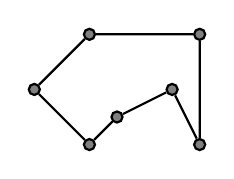
\begin{tikzpicture}[thick,scale=0.35]
    \plotpoints
    \draw (a) -- (b) -- (c) -- (e) -- (d)  -- (f) -- (g) -- (a);
  \end{tikzpicture}

  \bigskip

  Tour
  \[
    c(\text{Tour})\leq 2 \cdot c(MST)
  \]

\end{columns}

\begin{center}
  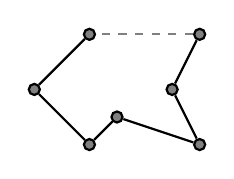
\begin{tikzpicture}[thick,scale=0.35]
    \plotpoints
    \draw (g) -- (a) -- (b) -- (c) -- (d) -- (e) -- (f);
    \draw[color=gray,dashed] (f) -- (g);
  \end{tikzpicture}

\bigskip
  
  $\text{OPT} \rightarrow \text{ST}$
\end{center}

\end{frame}




\begin{frame}
\begin{framed}
Double tree algorithm:
\medskip
\begin{enumerate}
\item $T\leftarrow \text{MST}$
\item {\color{red} Double all edges} in $T$
\item  $E_{tour} \leftarrow$ Euler tour
\item $\text{Tour}\leftarrow$ vertices in order of appearance in $E_{tour}$
\end{enumerate}
\end{framed}

\bigskip

\begin{framed}
  \medskip
  Christofide's algorithm:
\begin{enumerate}
\item $T\leftarrow MST$
\item  Add {\color{red} minimum perfect matching} of odd degree vertices in
  $T$
\item $E_{tour}\leftarrow$ Euler tour
\item $\text{Tour} \leftarrow $ vertices in order of appearance in $E_{tour}$
\end{enumerate}
\end{framed}
\end{frame}





\begin{frame}

\frametitle{Approximation Algorithms}
\framesubtitle{A $3/2$-approximation algorithm for Metric TSP: Christofides}

\bigskip

\begin{columns}[T,onlytextwidth]
  \column{0.3\textwidth}
  \centering
  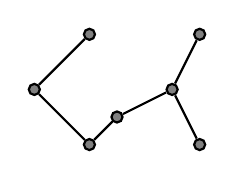
\begin{tikzpicture}[thick,scale=0.35]
    \plotpoints
    \draw (a) -- (b) -- (c) -- (e) -- (d);
    \draw (e) -- (f);
    \draw (a) -- (g);
    \end{tikzpicture}

  \column{0.3\textwidth}
  \centering
  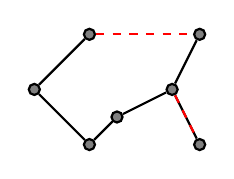
\begin{tikzpicture}[thick,scale=0.35]
    \plotpoints
    \draw (a) -- (b) -- (c) -- (e) -- (d);
    \draw (e) -- (f);
    \draw (a) -- (g);
    \draw[dashed,color=red] (g) -- (f);
    \draw[dashed,color=red] (e) -- (d);
  \end{tikzpicture}
  $$
    c(M) \leq \frac12 \text{OPT}:
  $$
  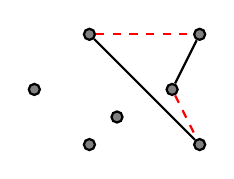
\begin{tikzpicture}[thick,scale=0.35]
    \plotpoints
    \draw (g) -- (d);
    \draw (e) -- (f);
    \draw[dashed,color=red] (g) -- (f);
    \draw[dashed,color=red] (e) -- (d);
  \end{tikzpicture}
  $$
    c(M) \leq \frac12 c(\text{Tour}) \leq c(\text{Tour}) \leq c(\text{OPT})
  $$
  
  \column{0.3\textwidth}
  \centering
  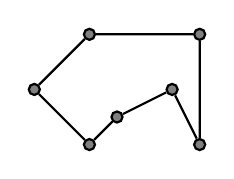
\begin{tikzpicture}[thick,scale=0.35]
    \plotpoints
    \draw (a) -- (b) -- (c) -- (e) -- (d)  -- (f) -- (g) -- (a);
  \end{tikzpicture}
\end{columns}

\bigskip

\end{frame}



\begin{frame}

  \frametitle{Approximation Algorithms}
\framesubtitle{Lower bounds}

  \begin{theorem}
For $\alpha<\frac{185}{184}$, there is no
$\alpha$-approximation algorithm for Metric TSP.
  \end{theorem}

\bigskip

  \begin{theorem}
There is no approximation algorithm for general TSP.
  \end{theorem}


\end{frame}




\begin{frame}
\frametitle{Local Search}

\begin{columns}[T,onlytextwidth]
\column{0.33\textwidth}
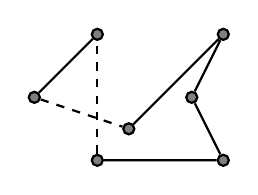
\begin{tikzpicture}[thick,scale=0.4]
  \plotpoints
  \draw (g) -- (a);
  \draw (b) -- (d) -- (e) -- (f) -- (c) ;
  \draw[dashed] (b) -- (g);
  \draw[dashed] (a) -- (c);
\end{tikzpicture}

\column{0.33\textwidth}
  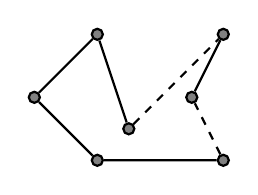
\begin{tikzpicture}[thick,scale=0.4]
    \plotpoints
    \draw[] (a) -- (b) -- (d);
    \draw (e) -- (f);
    \draw (c) -- (g) -- (a);
     \draw[dashed] (d) -- (e);
     \draw[dashed] (c) -- (f);
\end{tikzpicture}

 \column{0.33\textwidth}
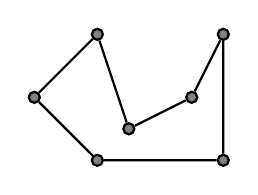
\begin{tikzpicture}[thick,scale=0.4]
\plotpoints
\draw[] (a) -- (b) -- (d) -- (f) -- (e) -- (c)
     -- (g) -- (a);
\end{tikzpicture}
\end{columns}
\end{frame}



\begin{frame}%%%%%%%%%%%%%%%%%%%%%%%%%%%%%%%%%%%%%%%%%%%%%%%%%%%%%%%%%%%%%%%%%%

\frametitle{Metaheuristics}

Trying different changes / accepting worsening changes:

\bigskip

\begin{columns}[T,onlytextwidth]
  \column{0.33\textwidth}
  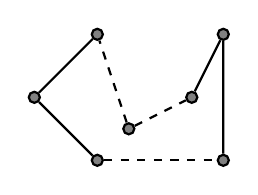
\begin{tikzpicture}[thick,scale=0.4]
    \plotpoints
    \draw[] (a) -- (b);
    \draw (d) -- (f) -- (e);
    \draw (g) -- (a);
    \draw[dashed] (b) -- (d);
    \draw[dashed] (c) -- (e);
    \draw[dashed] (c) -- (g);
  \end{tikzpicture}

  \column{0.33\textwidth}
  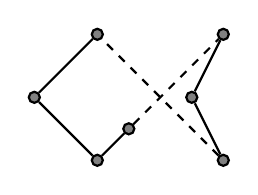
\begin{tikzpicture}[thick,scale=0.4]
    \plotpoints
    \draw[] (a) -- (b) -- (c);
    \draw (f) -- (e) -- (d);
    \draw (g) -- (a);
    \draw[dashed] (c) -- (f);
    \draw[dashed] (d) -- (g);
  \end{tikzpicture}

  \column{0.33\textwidth}
  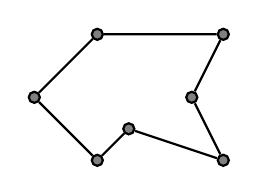
\begin{tikzpicture}[thick,scale=0.4]
    \plotpoints
    \draw[] (a) -- (b) -- (c) -- (d) -- (e) -- (f) -- (g) -- (a);
  \end{tikzpicture}
\end{columns}
\end{frame}
\begin{frame}%%%%%%%%%%%%%%%%%%%%%%%%%%%%%%%%%%%%%%%%%%%%%%%%%%%%%%%%%%%%%%%%%%

\frametitle{Contents}

\begin{table}
  \centering
\begin{tabular}{l|c c}
  &Approx Algorithms&Local Search + Metaheuristics\\[2mm]
\hline\\[-2mm]
Set Cover&\Checkmark&\\
Satisfiability&\Checkmark&\Checkmark\\
Traveling Salesman&\Checkmark&\Checkmark\\
Scheduling&\Checkmark&\Checkmark\\
Knapsack&\Checkmark&\\
Bin packing&\Checkmark&
\end{tabular}
\end{table}
  
\end{frame}


\againframe{firstpage}

\end{document}










\begin{frame}
  \frametitle{Assessment}

\medskip

\begin{itemize}

\itemsep=3ex

\item  Two {\alert{practical project assignments}}
  (include programming in Python)

\item {\alert{Oral exam}} based on:
  \begin{itemize}

  \item the theoretical part
  \item the two assignments
  \end{itemize}
Grading by the Danish 7-mark
scale w.\ external examiner\\ Exam aids allowed.
\end{itemize}
\end{frame}



